\documentclass[10pt,a4paper]{article}
\usepackage[utf8]{inputenc}
\usepackage[danish]{babel}
\usepackage{amsmath}
\usepackage{amsfonts}
\usepackage{amssymb}
\usepackage{graphicx}
\usepackage[left=2cm,right=2cm,top=2cm,bottom=2cm]{geometry}


\usepackage{titlepic}
\usepackage{enumerate}
\usepackage{enumitem}
\usepackage{float}
\usepackage{pdfpages}
\usepackage[colorlinks = true,
            linkcolor = blue,
            urlcolor  = blue,
            citecolor = blue,
            anchorcolor = blue]{hyperref}
\usepackage[explicit]{titlesec}
\usepackage{pstricks}
\usepackage[amsmath,thmmarks]{ntheorem} %pakke til at lave sætningsenvorinmets (kan ikke loades sammen med amsthm)
\usepackage{color}
\usepackage{tikz}

%opretter environmets til sætningsstrukturen 
\theorembodyfont{\normalfont}

	
	%sætnings environment	
	\newtheorem{thm}{Sætning}

	\theoremstyle{break}	
	%opgave environment	
	\newtheorem{opg}{Opgave}	

	%Korrolar environment
	\newtheorem{korollar}[thm]{Korollar}	
	
	%Lemma environment	
	\newtheorem{lemma}[thm]{Lemma}
	
	\theoremsymbol{\ensuremath{\circ}}	
	
	%definition environment	
	\newtheorem{definition}[thm]{Definition}
	
	%eksempel environment	
	\newtheorem{eksempel}[thm]{Eksempel}
	
	
	
	%Bevis environment
	\theoremstyle{nonumberplain}
	\theoremheaderfont{%
	\normalfont\itshape}
	\theorembodyfont{\normalfont}
	\theoremsymbol{\ensuremath{\square}}
	\theoremseparator{.}
	
	\newtheorem{proof}{Bevis}
	\newtheorem{los}{Løsning}
	






\setlength\parindent{0pt}

%\titleformat{\section}{\Large\bfseries}{}{0pt}{#1}
%\titleformat{\subsection}{\large\bfseries}{}{0pt}{#1}


%nye komandoer
\newcommand{\mR}{\mathbb{R}}
\newcommand{\mZ}{\mathbb{Z}}
\newcommand{\mN}{\mathbb{N}}
\newcommand{\mQ}{\mathbb{Q}}
\newcommand{\mC}{\mathbb{C}}
\newcommand{\hs}{\hspace{2mm}}
\newcommand{\Hs}{\hspace{4mm}}
\newcommand{\pipe}{\hs | \hs}
\newcommand{\lp}{\left(}
\newcommand{\rp}{\right)}
\newcommand{\vect}[1]{\underline{#1}}
\newcommand{\matr}[1]{\underline{\underline{#1}}}
\newcommand{\cnum}[1]{\raisebox{.5pt}{\textcircled{\raisebox{-.9pt} {#1}}}}




\author{Mikkel B. Goldschmidt}
\title{Synopser til Kemi A mundtlig eksamen}
\date{\today}



\begin{document}
\maketitle
\tableofcontents
\pagebreak

\section{Syrer og baser – identifikation af svag og stærk syre}

\pagebreak


\section{Syrer og baser – phosphorsyre i cola}

\pagebreak


\section{Syrer og baser – Bjerrumdiagram}

\pagebreak


\section{Organisk kemi – spektroskopi}

\pagebreak


\section{Organisk kemi – syntese}

\pagebreak


\section{Organisk kemi – identifikation (Cellulosefortynder)}

\pagebreak

\section{Organisk kemi – identifikation (Oxidation af alkoholer)}

\pagebreak


\section{Farvestoffer – farveindholdet i sodavand}
\textbf{Spørgsmål}\\
Med udgangspunkt i eksperiment ”Farvestofindholdet i sodavand” skal du redegøre for, hvorledes man i praksis kan bestemme farvestofindholdet i en sodavand. 

I din gennemgang kan du gøre brug af nedenstående stikord. 

I din besvarelse skal bilagene inddrages.


\vspace{0.5 cm}
\textbf{Stikord}\\
Lambert-Beers lov, farvedannelse i organiske molekyler, orbitaler og hybridisering.

\section*{Synopsis}

\subsection{Farvedannelse i organiske molekyler}
Organiske molekyler tager farve af flere forskellige ting.
Primært tager de farve når der dannes en delokaliseret elektronsky rundt om molekylet. 

\paragraph{Kojugerede dobbeltbindinger} er en af de ting der kan danne en delokaliseret elektronsky. 
Konjugerede dobbeltbindinger er skiftende dobbelt- og enkeltbindinger mellem carbonatomer. 
Normalt skal der minimum være 8 konjugerede dobbeltbindinger for at der opstår farve (se side 178 B).

\paragraph{Chromofore grupper} er en anden ting der kan ændre farven på et molekyle. 
Disse er grupper med et eller to ledige elektronpar, der derfor giver anledning til en forskydning af elektronskyen. 
Når disse grupper er til stede, kan der opstå farve med færre konjugerede dobbeltbindinger (se side 180 B).
Disse er eksempelvis:
\begin{figure}[h]
    \centering
    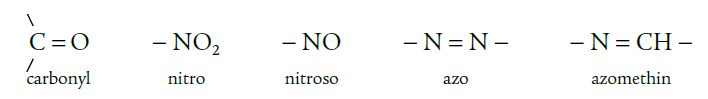
\includegraphics[scale=0.7]{Figurer/chromoforeGrupper}
    \caption{Eksempler på chromofore grupper. Fra side 180 B}
\end{figure}


\paragraph{Auxochrome (farvemodificerende) grupper} kan ændre farven og intensiteten af farven på et organisk molekyle. 
Disse grupper er eksempelvis:
\begin{figure}[h]
    \centering
    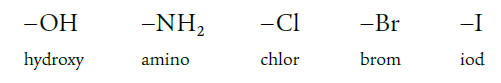
\includegraphics[scale=.7]{Figurer/auxochromeGrupper}
    \caption{Eksempler på auxochrome grupper. Fra side 180 B.}
\end{figure}
På side 181 B ses hvordan indigo med tilførsel af 2 $-Br$ grupper bliver til purpur.


\subsection{Måling af farve}
\subsubsection{Absorbans}
Absorbans beskriver hvor meget et stof absorberer af en bestemt farve.
Vi måler arbsorbans som andelen af en intensitet der bliver absorberet af en opløsning på følgende måde:
$$A=\log(\frac{I_0}{I})$$
Her beskriver $A$ absorbansen, $I_0$ den intensitet der slipper igennem opløsningsmidlet alene og $I$ den intensitet der slipper igennem af opløsningen.
De illustreres meget godt på følgende figur:
\begin{figure}[h]
    \centering
    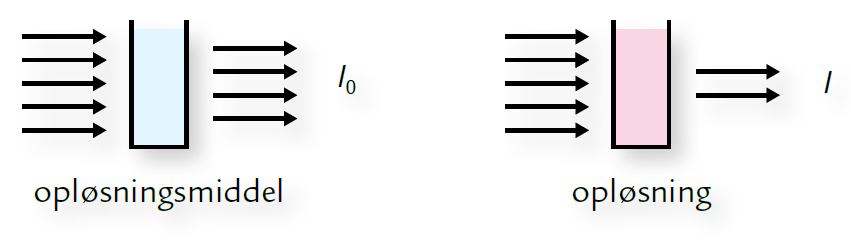
\includegraphics[scale=0.4]{Figurer/intensitet}
    \caption{Intensiteten $I_0$ er mindre da en del af den bliver absorberet i den farvede opløsning. Side 184 B.}
\end{figure}

\subsubsection{Lambert-Beers lov}
Beskrivelse af Lambert-Beers lov. 
$$ A= \varepsilon_\lambda \cdot [S] \cdot l  $$
$A$ er absorbans, $[S]$ er aktuel stofmængdekoncentration af stof S, $l$ er kuvettebredden og $= \varepsilon_\lambda$ er arbsorbtionskoefficenten.

\subsection{Bestemmelse af farvestofindhold i sodavand}
\subsubsection{Et enkelt farvestof}
\begin{enumerate}
    \item Bestem den maksimale absorbtionsbølgelængde (herfra kaldet $\lambda_{max}$ ved at lave et fuldspektrum.
    
    \item Bestem $\varepsilon_{\lambda_{max}}$) ved at måle sammenhørende værdier af $[S]$ og $A$ med et kendt $l$.
    
    \item Bestem $A$ ved $\lambda_{max}$ en kendt koncentration af sodavand og udnyt den kendte værdi af $\varepsilon_{\lambda_{max}}$ til at bestemme koncentrationen af favestoffet.  
\end{enumerate}

\subsection{To farvestoffer}
Gennemgås ikke med mindre at de spørger om det.

\pagebreak


\section{Farvestoffer – fremstilling af indigo og indfarvning}

\pagebreak


\section{Hastighed – reaktionsorden}
\textbf{Spørgsmål}\\
Med udgangspunkt i en gennemgang af eksperiment ”Affarvning af krystalviolet” skal du redegøre for, hvorledes man i praksis kan bestemme reaktionsorden for en kemisk reaktion. 

I din gennemgang skal du inddrage nogle af nedenstående stikord. 

I din besvarelse skal bilagene inddrages.

\vspace{0.5 cm}
\textbf{Stikord}\\
Reaktionshastighed, reaktionsorden, hastighedskonstant, halveringstid, elementarreaktioner og aktiveringsenergi.

\subsection*{Synopsis}

\pagebreak


\section{Hastighed – aktiveringsenergi}

\pagebreak


\section{Hastighed – enzymkinetik}

\pagebreak


\section{Termodynamik – reaktionsentalpi}

\pagebreak


\section{Termodynamik – Van’t Hoffs ligning}

\pagebreak

\section{Redoxreaktioner}

\pagebreak


\section{Redoxreaktioner - jernindhold i ståluld}
\textbf{Spørgsmål}\\
Med udgangspunkt i eksperiment ”Bestemmelse af jernindholdet i ståluld” skal du redegøre for, hvorledes man i praksis kan bestemme indholdet af jern i ståluld og indstilling af kaliumpermanganat opløsning.

I din gennemgang kan du gøre brug af nedenstående stikord. 

I din besvarelse skal bilagene inddrages.

\vspace{0.5 cm}
\textbf{Stikord}\\
Reduktion, oxidation, oxidationstal, afstemning af redoxreaktioner og masseprocent.

\section*{Synopsis}
\newcommand{\RNum}[1]{\textit{\uppercase\expandafter{\romannumeral #1\relax}}}
Alle udregninger ligger i et Maple dokument i datamappen for dette forsøg.

\subsection{Bestemmelse af $MnO_4^-$'s koncentration}
\subsubsection{Afstemning af redoxreaktion}
Ved sammenblanding med oxalat ($C_2O_4^{2-}$) fra natriumoxalat ($Na_2C_2O_4$) sker følgende reaktion:
$$MnO_4^- + C_2 O_4 ^{2-} \rightarrow Mn^{2+} + CO_2$$
Denne afstemmes som redoxreaktion. 
Først bestemmes oxidationstal:
$$\overset{+\RNum{7}}{Mn}O_4^- + \overset{+\RNum{3}}{C_2} O_4 ^{2-} \rightarrow \overset{+\RNum{2}}{Mn^{2+}} + \overset{+\RNum{4}}{C}O_2$$

Ved at kigge på ændring i oxidationstal får vi da:
$$Mn: 5\downarrow$$
$$ C: 1\uparrow$$
For at få samlet ændring på $0$ på begge sider, tager vi 5 af hvert carbon. 
Da vi har en reaktant med 2 carbon per molekyle bliver vi dog nødt til at gange hele reaktionen med 2, da vi ellers skulle have $\frac{5}{2}$ oxalat:
$$2\space{} MnO_4^- + 5 C_2 O_4 ^{2-} \rightarrow 2 Mn^{2+} + 10 CO_2$$
Vi ser nu en samlet ladning på $-12$ hos reaktanterne og en samlet ladning på $+4$ hos produkterne. 
Dermed er der en ladningsforskel på 16. 
Da reaktionen foregår sammen med svovlsyre, kan der tilføres 16 $H^+$ hos reaktanterne og tilsvarende 8 $H_2 O$ hos produkterne. 
$$16 H^+ + 2 MnO_4^- + 5 C_2 O_4 ^{2-} \rightarrow 2 Mn^{2+} + 10 CO_2 + 8 H_2 O$$
Hvis man tæller O'er på begge sider ser man nu at reaktionen stemmer overens. 
Dermed er redoxreaktionen afstemt. 

\subsubsection{Titrering med $MnO_4^{-}$ på $Na_2C_2O_4$}
Da $MnO_4^{2-}$ har en markant pink farve, vil den kunne ses hvis ikke den reagerer med $C_2O_4^{-}$ hvor den i stedet bliver til den farveløse $Mn^{2+}$ jvf. reaktionen i forrige afsnit. 
I udregningsdokumentet ses hvordan koncentrationen af $KMnO_4$ bestemmes fra det tilsatte volumen.

\subsection{Bestemmelse af jernindhold i ståluld}
\subsubsection{Reaktion mellem svovlsyre ($H_2 SO_4$) og jern}
Den første del af forsøget hvor jernindholdet bestemmes, handler om at få fjernet jernet fra stålulden. 
Dette gøres det ved at lægge det i stærk svovlssyre(2M) natten over. 
Da sker følgende reaktion:
$$  Fe + 2 H^+ \rightarrow Fe^{2+} + H_2  $$
Reaktionen forløber kun fordi jern ikke er et ædelmetal, og det står derfor før H i spændingsrækken ("Hvis metallet står før ionen - så forløber reaktionen").

\subsubsection{Reaktion mellem $Fe(II)$ og $MnO_4^-$}
Her sker igen en redoxreaktion.
Den afstemte ser sådan her ud, og selve afstemningen er ret standard. 
Bemærk at der stadig er svovlsyre i opløsningen, hvorfor der tilføjes passende $H^+$:
$$ 8H^+ + 5 Fe^{2+} + MnO_4^- \rightarrow Mn^{2+} + 5 Fe^{3+} + 4 H_2O $$
Da vi kender koncentrationen af $MnO_4^-$ fra bestemmelse i forrige afsnit, og vi ved hvornår vi har brugt alt jernet op fra at opløsningen tager farve (da der er $MnO_4^-$ i den hvis det ikke reagerer med jernet), kan vi bestemme stofmængden af jern som 5 gange så stor som den tilsatte mængde $MnO_4^-$.
\pagebreak


\section{Kemiske ligevægte}


\end{document}
